%%%%%%%%%%%%%%%%%%%%%%%%%%%%%%%%%%%%%%%%%%%%%%%%%%%%%%%%%%%%%%%%%%%%%%%%%%%%%%%%
%        Diploma project template - (C) Balan Mihail-Alexandru, 2009           %
%%%%%%%%%%%%%%%%%%%%%%%%%%%%%%%%%%%%%%%%%%%%%%%%%%%%%%%%%%%%%%%%%%%%%%%%%%%%%%%%

% Print on A4 paper, double-sided, base font size 12pt
%\documentclass[a4paper,12pt,twoside,draft]{report}
\documentclass[a4paper,12pt,twoside]{report}

\usepackage{titlesec}

\titlespacing*{\section}
{0pt}{5.5ex plus 1ex minus .2ex}{4.3ex plus .2ex}
\titlespacing*{\subsection}
{0pt}{5.5ex plus 1ex minus .2ex}{4.3ex plus .2ex}

\usepackage{listings}


\lstset{ %
  backgroundcolor=\color{white},   % choose the background color; you must add \usepackage{color} or \usepackage{xcolor}; should come as last argument
  basicstyle=\fontsize{8}{11}\ttfamily,        % the size of the fonts that are used for the code
  breakatwhitespace=false,         % sets if automatic breaks should only happen at whitespace
  breaklines=true,                 % sets automatic line breaking
  captionpos=b,                    % sets the caption-position to bottom
  deletekeywords={...},            % if you want to delete keywords from the given language
  escapeinside={\%*}{*)},          % if you want to add LaTeX within your code
  extendedchars=true,              % lets you use non-ASCII characters; for 8-bits encodings only, does not work with UTF-8
  frame=single,	                   % adds a frame around the code
  keepspaces=true,                 % keeps spaces in text, useful for keeping indentation of code (possibly needs columns=flexible)
  keywordstyle=\color{blue},       % keyword style
  language=Python,                 % the language of the code
  morekeywords={*,...},            % if you want to add more keywords to the set
  numbers=left,                    % where to put the line-numbers; possible values are (none, left, right)
  numbersep=5pt,                   % how far the line-numbers are from the code
  numberstyle=\color{black}, % the style that is used for the line-numbers
  rulecolor=\color{black},         % if not set, the frame-color may be changed on line-breaks within not-black text (e.g. comments (green here))
  showspaces=false,                % show spaces everywhere adding particular underscores; it overrides 'showstringspaces'
  showstringspaces=false,          % underline spaces within strings only
  showtabs=false,                  % show tabs within strings adding particular underscores
  stepnumber=2,                    % the step between two line-numbers. If it's 1, each line will be numbered
  stringstyle=\color{black},     % string literal style
  tabsize=2,	                   % sets default tabsize to 2 spaces
  title=\lstname                   % show the filename of files included with \lstinputlisting; also try caption instead of title
}
% \usepackage[top=3.81cm,bottom=3cm,left=3.5cm,right=2.54cm]{geometry}
\usepackage[top=3.81cm,bottom=3cm,inner=3cm,outer=2.54cm]{geometry}

% Actual font selection
\usepackage{pxfonts} % bookman | pxfonts | cmbright

% Include support for romanian hyphenation (if installed on your sistem)
% \usepackage[romanian]{babel}

% Include support for correct printing of romanian characters
\usepackage[T1]{fontenc}
\usepackage{ucs}
\usepackage[utf8x]{inputenc}

% Include support for graphics
\usepackage[pdftex]{color,graphicx}

% Include support for hyperlinks in the document
\usepackage{hyperref}
\hypersetup{unicode=true,%
	colorlinks=true,%
	citecolor=black,%
	filecolor=black,%
	linkcolor=black,%
	urlcolor=blue}

\setcounter{tocdepth}{3}

% remove default paragraph indentation
% \setlength{\parindent}{0pt}
\usepackage{parskip}

% Describing algorithms
\usepackage[figure,longend,lined,boxed]{algorithm2e}
% \usepackage{algorithmic}

% Settings for using source highlighter
\usepackage{alltt}
\usepackage{marvosym}

\newcommand{\hlstd}[1]{\textcolor[rgb]{0,0,0}{#1}}
\newcommand{\hlnum}[1]{\textcolor[rgb]{0.53,0,0.13}{#1}}
\newcommand{\hlesc}[1]{\textcolor[rgb]{1,0,1}{\bf{#1}}}
\newcommand{\hlstr}[1]{\textcolor[rgb]{0.67,0.27,0}{#1}}
\newcommand{\hldstr}[1]{\textcolor[rgb]{0,0.53,0}{#1}}
\newcommand{\hlslc}[1]{\textcolor[rgb]{0.93,0.47,0}{#1}}
\newcommand{\hlcom}[1]{\textcolor[rgb]{1,0.53,0}{#1}}
\newcommand{\hldir}[1]{\textcolor[rgb]{0,0.53,0.27}{\bf{#1}}}
\newcommand{\hlsym}[1]{\textcolor[rgb]{0,0,0}{\bf{#1}}}
\newcommand{\hlline}[1]{\textcolor[rgb]{0.2,0.2,0.2}{#1}}
\newcommand{\hlkwa}[1]{\textcolor[rgb]{0.4,0.07,0.07}{\bf{#1}}}
\newcommand{\hlkwb}[1]{\textcolor[rgb]{0,0,0.4}{\bf{#1}}}
\newcommand{\hlkwc}[1]{\textcolor[rgb]{0,0,0.4}{#1}}
\newcommand{\hlkwd}[1]{\textcolor[rgb]{0,0.27,0.4}{#1}}
\definecolor{bgcolor}{rgb}{1,1,1}

% Setup some new commands for easier image inserting and figure referencing
% Creates the text for referring to the figure identified by the key given as
% the first argument.
\newcommand{\figname}[1]{\emph{figura \ref{#1}}}

% Inserts a new figure, with these parameters:
%	#1 - filename of the figure to be inserted
%	#2 - caption for the figure
%	#3 - label for the figure (used in \ref-ing the figure)
\newcommand{\insfig}[3]{
	\begin{figure}[!htb]
		\begin{center}
			\fbox{
				%\includegraphics[width=0.75\textwidth]{#1}
 				\includegraphics{#1}
			}
			\caption{#2\label{#3}}
			
	    \end{center}
	\end{figure}
}

% Inserts a new figure, with these parameters:
%	#1 - filename of the figure to be inserted
%	#2 - caption for the figure
%	#3 - label for the figure (used in \ref-ing the figure)
%	#4 - fraction of the text width occupied by the figure
\newcommand{\insfigw}[4]{
	\begin{figure}[!htb]
		\begin{center}
			\fbox{
				\includegraphics[width=#4\textwidth]{#1}
			}
			\caption{#2\label{#3}}
			
	    \end{center}
	\end{figure}
}

% Inserts a new figure, with these parameters:
%	#1 - filename of the figure to be inserted
%	#2 - caption for the figure
%	#3 - caption for display in the list of figures
%	#4 - label for the figure (used in \ref-ing the figure)
%	#5 - fraction of the text width occupied by the figure
\newcommand{\insfigshw}[5]{
	\begin{figure}[!htb]
		\begin{center}
			\fbox{
				\includegraphics[width=#5\textwidth]{#1}
			}
			\caption[#3]{#2\label{#4}}
			
	    \end{center}
	\end{figure}
}

% Setting headers
\usepackage{fancyhdr}
\pagestyle{fancy}
\fancyhead{}
\fancyhead[LE]{\nouppercase{\leftmark}}
% \fancyhead[RO]{\nouppercase{\rightmark}}

% Set spacing at 1.5lines
\linespread{1.3}

% Document begins here
\begin{document}

% Create title page
\documentclass{article}

\title{Introduction}
\author{Andrei-Ciprian Dobre}

\begin{document}
	\maketitle
	\newpage
\end{document}

% Leave a blank page for double side printing
\thispagestyle{empty}
\newpage
\hbox{}

% insert the table of contents
\tableofcontents
\newpage

\chapter{Introduction}

Following the massive expansion of embedded systems led by smart devices, a new inevitable trend began to develop. The automotive industry started to embed more and more computational power in the ubiquitous personal car. Automotive specific Linux operating systems  became unavoidable. For this particular reason a few projects started to emerge that aimed to shape the future development efforts towards a maintainable, safe and uniform ecosystem. They are initiatives started by colossal companies whose main line of activity is not related to software but understood the importance of a high quality software component.

While automotive giants discussed how to better approach a future of connected cars, the Linux Foundation came with a proposition - a specification for Automotive Grade Linux (AGL). AGL is intended to be a distribution that serves as a standard of quality. It follows the model of an earlier, very successful specification, the Carrier Grade Linux.

In a context of ever expanding embedded computer networks and the emergence of new specifications and standards, the Linux ecosystem is still lacking open source tools that facilitate testing. While a lot of effort is directed towards specialized and efficient testing tools, there is currently no solution that offers a full image about the compliance of a distribution with a specification. This paper describes a framework proposal for this particular task - validate a whole Linux distribution based on a given specification. The framework aims to contribute to an efficient, well thought and safe embedded Linux ecosystem by reducing the development effort through automation. It anticipates an increase of Linux distribution or application vendors and tries to enable a community-driven effort towards higher standards that will ultimately benefit the end-users.

For convenience, the framework proposal will also be referred to as "Ellida", the name chosen for the software implementation.\footnote{In the old Norse culture, Ellida is the name of a magical ship offered to the Vikings by the gods - the first Viking dragon ship.}


\chapter{Background}

\section{Linux testing}

The Linux ecosystem has been around for a long time and as a consequence, every new version inherits a vast codebase. Being an open source system it heavily relies on the community to validate the functionality and improve it along the way. The bugs are mainly reported by the users, but by the time the new software reaches end user the bug might be much more difficult to fix. To ease the work of developers automated testing suites emerged that validated subsystems and provided continuous integration.

Ideally, a developer would test the new code as early as possible - before submitting the patch. However, such early testing is usually not extensive or rigorous enough and might not happen at all. Untested patches often lead to notable developer effort wasted on bugs that are found later in the cycle when it is significantly less efficient to fix them.

Several large projects developed over time to automate the Linux Kernel testing such as LTP - Linux Testing Project and Autotest. However, testing for compliance is currently done inside companies that provide distributions for the IT industry, such examples are Wind River and MontaVista. This embedded software vendors use in-house, closed source validators, yet the profiler characteristics are made public so that clients benefit from the transparency of the testing process. For instance, Wind River provides a carrier grade profile for their Linux distributions so clients can see how the system they intend to purchase was validated. This information can be used for creating a open-source tool with the same purpose that can have a larger impact.

\section{Linux distributions and specifications}

Each specification aims to provide a guideline for future developers and tries to shape and direct a specific technological branch so that future development is not hindered in any way, is secure and based on sound principles. A specification usually consists of a set of rules, guidelines and principles. They can ease the development and maintenance effort of the whole community by bringing uniformity and structure to the systems it is used for. It is intended to be as extensive as possible but there is a natural limitation to how much a specification can cover. Usually they focus on a very specific system that is part of a larger branch. This focus makes the specification easier to implement and ensures a more detailed coverage and higher quality. The present paper discusses only the software specifications created for production-ready Linux distributions.

\subsection{The Yocto Project}
The Yocto Project is an open source collaboration project that aims to facilitate creation of embedded Linux distributions. The project relies heavily on previous work done in different open source communities. It brings together tools and a template system to allow the creation of custom Linux based operating systems. Because Yocto has a very broad approach and the purpose of creating a whole distribution is difficult to achieve, a reference Yocto distribution was created called \textbf{Poky}. In itself, Yocto only states that a custom image must be created based on a template and aims to facilitate interoperability between the tools under the project umbrella, Poky offers a concrete implementation of this idea. It offers a simple yet comprehensive example of how Yocto is supposed to work and can be used for fast prototyping. The main components of Poky are \textbf{BitBake}, \textbf{OpenEmbedded Core} and Yocto specific metadata. The proposed framework is integrated with Poky and uses its subsystems to provide the testing functionality.

\subsubsection*{Bitbake}
Bitbake is a cross-compilation tool able to parse Python and Shell scripts. It is inspired by the package management system used in Gentoo Linux distribution - Portage. Bitbake uses a system of recipes to keep track of the required packages and the dependencies between them. The recipes provide the template system of Yocto, they are the main input data based on witch a custom distribution is created. Since Bitbake is able to fetch source code from most common repository types such as github and mercurial and install most common package formats such as .deb and .rpm, the available code base is extensive. It also means that as long as builds happen often, the software will be up to date.

Arguably Bitbake's greatest advantage is the dependency management of the tasks. After parsing the recipes (which can be a combination of Python and Shell script) Bitbake is able to create concurrent tasks that process operations such as code fetching, building and installing and order them based on their dependencies. Considering how large a single build of Poky can become (over 24GB) the efficiency of Bitbake makes the system viable.

\subsubsection*{OpenEmbedded Core}
OpenEmbedded (OE) is an open source project that pre-dates Yocto and is based on Bitbake recipes. After the creation of the Yocto Project, the community behind OpenEmbedded had the opportunity to change the architecture. In the beginning all the recipes of the system were all gathered in the same place, but the system became unmaintainable. The recipes were therefore split intro layers and the codebase of OE was split between OE-core and meta-oe. The core provides all the basic functionality required by anyone who tries to build an embedded distribution, while meta-oe contains all the rest of the recipes. OpenEmbedded project offers an extensive list of available layers.

By default, Poky contains the OE core, but it also preserves the layered architecture through which almost any common functionality, software and tools can be added. The proposed framework uses one such layer called meta-ellida to integrate with Yocto.

\subsection{CGL - Carrier Grade Linux}
The first of the two specifications discussed and supported by the framework is CGL - Carrier Grade Linux.
Given its broad approach, Carrier Grade Linux can be thought of as a convergence of other specifications. The original intent was to identify functionality already available in the open source community that is of particular interest to carriers. Most of the requirements laid out in the CGL specification apply equally well to systems ranging from large corporate infrastructures to small, highly mobile devices.

The CGL specification is very much requirement oriented. The structure follows a few abstract characteristics that a system should have and then specifies in great detail how these attributes can be achieved or at least tested. The main requirements of a carrier grade distribution are listed next.

\begin{enumerate}
\item \textbf{Standard}

The first section of the document addresses compliance with many other specifications or standards such as the Linux Standard Base (LSB), specific pieces of POSIX standards, IPv6 and IP Security standards (IPsec), Requests for Comment (RFCs), and PCI Express specifications.
\item \textbf{Hardware}

The hardware requirements describe hardware-specific support considered necessary for carrier environments.
\item \textbf{Serviceability}

The serviceability section develops on topics regarding the accessibility, remote maintenance and monitoring of possibly difficult to access systems. 
\item \textbf{Performance}

Performance wise, a number of attributes of the operating system that must be configurable at run-time are specified, along with process scheduling, signal processing order, priorities and methods for timely processing.
\item \textbf{Security}

The security segment aims to make systems more resistant to a wide range of attacks and increase the reliability. They cover aspects ranging from technical details such as avoiding buffer overflows to architectural and system wide facilities such as using access control and role-based access control or using technologies such as Trusted Platform Module.
\item \textbf{Availability}

The availability focuses on methods and features that lower the probability of having sudden or unexpected loss of functionality. Having a very high uptime is one of the vital aspects of a carrier system.
\item \textbf{Cluster}

The Cluster requirement category has a similar purpose to the Availability section, but instead of focusing on individual systems it refers to cluster based systems. It states the requirements for providing high availability using a multi-system cluster.

\end{enumerate}

Considering the scale and volatility of today's communications CGL proved to be of invaluable help. This is why the Linux Foundation has started setting the groundwork for standards and specifications that will hopefully guide other industrial branches. New IT industries are emerging around concepts such as smart cities and connected automotive products and they come with a highly disruptive potential. CGL's development paved the way for a multitude of standards and specifications that may help bring unity to a very dynamic, yet important factor of our life.

\subsection{AGL - Automotive Grade Linux}
The second specification discussed is relatively new and not yet as polished and mature as CGL, it aims to bring consistency to the automotive Linux ecosystem - AGL - Automotive Grade Linux. AGL is a Linux Foundation Collaborative Project that tries to provide the main automobile producers with a set of rules to follow when creating embedded distributions that run inside cars, but is also dedicated to creating open source software solutions for automotive applications. The initiative led to the creation of a reference Linux distribution based on Yocto. It enables rapid prototyping and is an opportunity for the industry players to collaborate towards a safer, more user-oriented software system. The AGL Workgroup has the support or several large vendors from the automotive and semiconductor industries.

The architecture of the specification is based on four layers. Each layer covers a separate part of the distribution and has rules concerning practical aspects of the system.

\begin{figure}[h!]
  \centering
	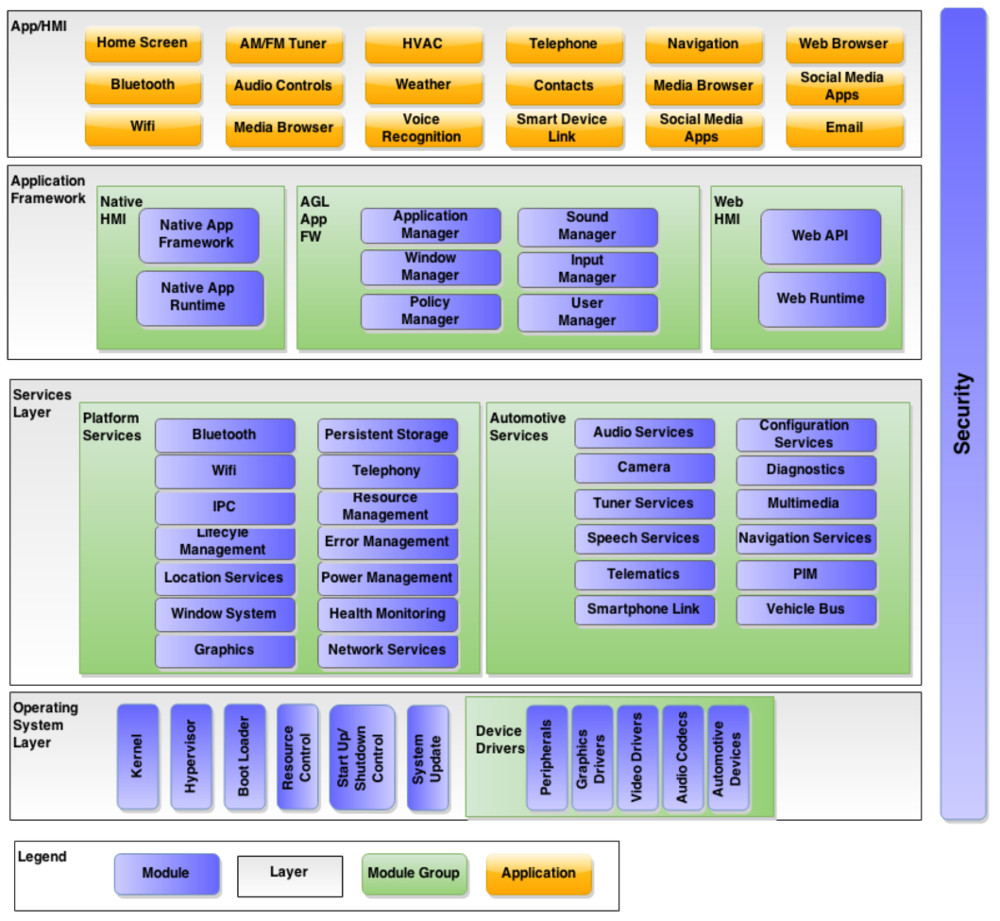
\includegraphics[width=0.9\textwidth]{images/agl_arch.jpg}
    \caption{AGL Architecture}
\end{figure}

\begin{enumerate}
\item \textbf{App/HMI}

The layer contains applications along with the business logic behind them and the human-machine interface (HMI). It is mainly comprised of guidelines regarding the user interface and the frameworks that link together the UI and the applications. 
\item \textbf{Application Framework}

The AGL Application Framework is meant to provide basic functionality to all applications regardless of the framework they were built with. It is intended to standardize \textbf{how} system-wide services are provided.
\item \textbf{Services}

The Services Layer contains user space services that all applications can access. It defines \textbf{which} services are available system-wide and their behaviour. Generally the services provide either an IPC type interface or a subroutine/function API.
\item \textbf{Security}

AGL only provides a very brief guide to security, stating only that a system-wide access control system should be in place.
\item \textbf{Operating system}

The OS layer deals with the more low level requirements of the system, regulating the behaviour of the memory, storage, file systems, kernel etc.
\end{enumerate}

AGL currently only targets In-Vehicle-Infotainment (IVI) systems, but additional use cases such as instrument clusters and telematics will eventually be supported. Linux Foundation expressed great interest in supporting and developing AGL over time. Therefore, it is not far-fetched to expect that it will have an impact in the embedded market and that testing tools will be in demand.

\subsubsection*{Pre-AGL initiatives - GENIVI}
Before 2012, when AGL collaborative open source project started bringing together automakers, another initiative with roughly the same purpose called GENIVI was created (2009). GENIVI is a non-profit industry alliance committed to driving the broad adoption of open source, In-Vehicle Infotainment (IVI) software and providing open technology for the connected car. GENIVI project currently maintains a fairly extensive list of open source applications created specifically for cars and benefits from both the support of a large community and sponsoring from large car manufacturers. GENIVI filled a gap in the automotive industry by pioneering the use of free and open source software for non-safety-critical automotive systems. It is currently more popular among European car makers, while AGL is being adopted by most Asian producers. However, considering the two to be competitors on the automotive market would not be very accurate. GENIVI applications can be used alongside or inside the AGL systems. They complete each other and strengthen the presence of open source software in a market where vendor specific products used to be ubiquitous. The effort to make reliable, secure and easy to use software while being cost effective and with a short time-to-market cycle has proven to be a hard limitation in all industries where software development is necessary. Therefore, AGL and GENIVI will have a wider impact by functioning alongside one another. The trend these initiatives started will not fade too soon and is creating a technological void.

\subsection{AGL - CGL comparison}
Even if the resulting set of guidelines are similar, the two specifications have different approaches. AGL has the software system as starting point and describes how it should behave in a broad sense. This is made obvious by the layered structure, with each layer being a part of the software system. CGL on the other hand has the requirements as starting point. It starts by defining what is important for the user or what is expected in abstract terms such as being reliable and secure. The specification then develops on each requirement through a set of rules and offers very detailed test scenarios along with the expected results. For the moment, AGL is still at version 1.0 and lacks a very formal structure, mainly because it is not intended to be used for a compliance program, but as a general guideline for the AGL project. CGL currently stands at the fifth version and has been in constant refining for almost 20 years. Since then, it has become a de facto standard for telecommunications providers. The comparison is relevant because it outlines how specifications might differ and how the framework's representation of them should be able to handle these differences.

\section{Related work}

\subsection{Fuego and AGL-JTA}
Fuego is the official automated test framework for the LTSI project. LTSI stands for Long Term Support Initiative and its purpose is to maintain a common Linux base for use in a variety of consumer electronics products. Fuego is a test framework specifically designed for embedded Linux testing, it uses a Jenkins front-end and a server-client model for running tests on multiple different boards at once. It also comes pre-packed with around 60 tests.

The main goals of Fuego are to facilitate community based testing by providing a simple system to run tests remotely and easily share both tests and results. These are achieved through hardware abstraction, the use of an extensible and user friendly front-end and the ability to use it as a hosted service. Even if Fuego has been around for a short time, and is still a work in progress, a branch called AGL-JTA was created for testing the official AGL distribution. The project is for the moment about a year old, has close to no documentation and exists in the form of a Fuego installation with certain plugin customisations and a small suite of tests.

Fuego and AGL-JTA are very close in purpose to the framework discussed. In truth, they can be used to offer the same functionality since they are meant to provide remote automatic software testing. However, Fuego is less focused on the high level functionality of full spec validation and more hardware oriented. Fuego is not dependent on Yocto generated systems although it supports Yocto, but instead has an architectural model that encapsulates hardware abstraction so that the LTSI kernels can be run on various boards. It also contains a custom built compile and schedule engine for running tests. These extensions, while providing relevant functionality, are cumbersome to use, increase the complexity a lot and are not mandatory for the task of validating distributions. The proposed frameworks aims to be hardware agnostic, it could as well use only VMs as long as they run the targeted distribution.

\begin{figure}[h!]
  \centering
	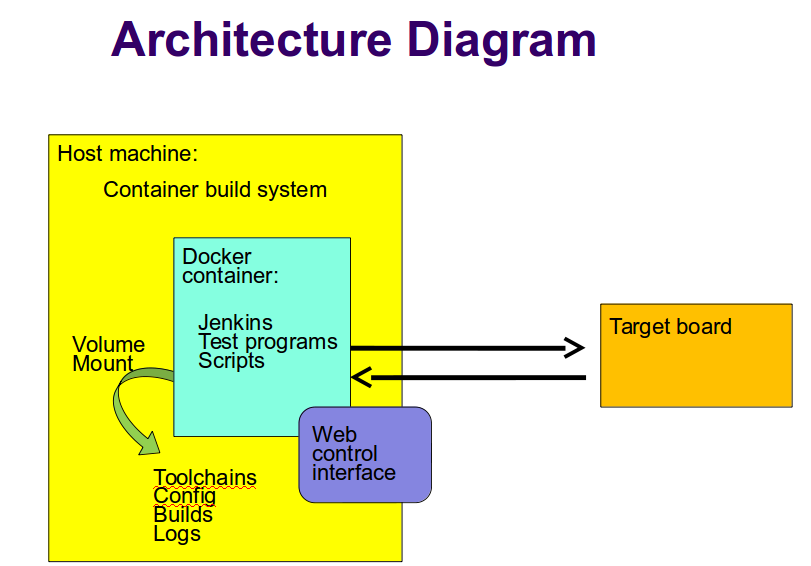
\includegraphics[width=0.7\textwidth]{images/fuego-arch.png}
    \caption{Fuego Architecture}
\end{figure}

\subsection{LAVA}

LAVA stands for Linaro Automation and Validation Architecture and is a continuous integration framework created by Linaro. It is intended to test OS - hardware configurations by installing operating systems on a variety of hardware, but can also install individual tests for in depth testing. LAVA can build and test kernels on supported hardware with a pre-set frequency and is designed for validation during development, thus the label of continuous integration. LAVA has features such as parallel scheduling, hardware sharing, live result reporting among others. The proposed framework tries to match the versatility and scalability of LAVA. 
\subsection{LTP}

The Linux Test Project is an open source project that has the support of companies such as IBM, Cisco, Fujitsu, SUSE, Red Hat. It aims to deliver test suites that validate Linux systems in terms of reliability, robustness, and stability. The LTP test suite contains a collection of tools - manly individual tests - that can be used for testing the Linux kernel and related features. The test collection consists of C programs and bash scripts that can be used either through CLI or through control files that define what tests should run. The C tests are automatically compiled and provide a very wide range of tests - over 4000 programs and scripts. Any testing framework should be able to harness this resource.


\chapter{Design}

\section{Providers}
A testing framework that aims to validate an entire distribution has far reaching requirements and should be capable to test mostly any software system while not hindering the testing process. To make it more probable that Ellida will be able to cover any aspect of a specification a model based on test providers was developed.

A \textbf{provider} is defined as a testing framework, tool or collection of tests focused on a specific subsystem or providing a specialised functionality. The providers are supported through classes that expose a uniform interface but abstract away the details such as executing specific files and parsing logs. Examples of providers are the LTP test suite, Image Tests - Yocto specific functionality that allows Python based unit tests to run through ssh, Lynis security auditing tool, Phoronix benchmarking platform, and LTTng tracing framework.

Specifications can be formally viewed as a set of categorized requirements as discussed in the abstraction section (\ref{specs}). Every category of requirements is usually specific to a particular subsystem or abstract attribute that the target system should have. Even if the abstract requirements are defined as categories and then split into more concrete, technical requirements, they still tend to be fairly vague, or leave room for interpretation.

The model proposed in the Ellida framework represents every such small technical requirement as a list of test sets, every set having a unique provider. A single requirement can therefore be tested with each and every provider while keeping the tests separated and organised on sets. A set can contain one or multiple tests, but requires that all tests are specific to the same provider. For example, the AGL.711 requirement can be validated by a list of two sets - A and B - with set A using the Core as provider and set B using LTP. The A set will contain one or more Python scripts while the B set will use LTP control files.

\begin{figure}[h!]
  \centering
	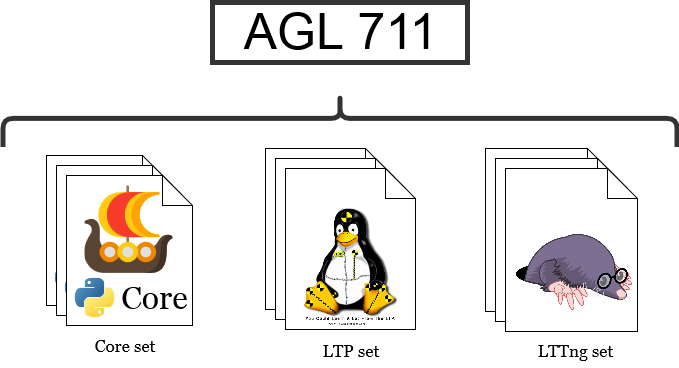
\includegraphics[width=0.6\textwidth]{images/providers.png}
    \caption{Validation based on multiple providers}
\end{figure}

\section{Specification abstraction and the test suite} \label{specs}
The specification representation is one of the important design features within the framework. The format has to be extensible, easy to use by both users and developers, with little or no constrains. The specifications consist of a folder tree structure that follows the underlying model of both AGL and CGL. The tree is populated with JSON files containing metadata relevant to each requirement.

Mirroring a specifications structure, a test suite uses the same format but further develops it to contain test files. Instead of having requirements as tree leafs, each requirement is a folder containing one or more sets. A set is just another folder with a provider specific structure whose only requirement is to contain a JSON document describing the set.

 
\begin{figure}[htb!]
	\begin{minipage}{0.48\textwidth} \centering
	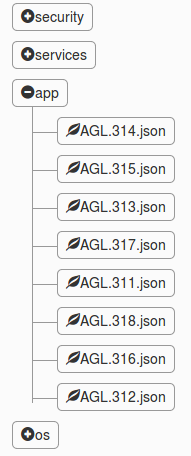
\includegraphics[width=0.5\linewidth]{images/agl_spec.png}
	\caption{AGL representation}
    \end{minipage} \hfill
    \begin{minipage}{0.48\textwidth} \centering
	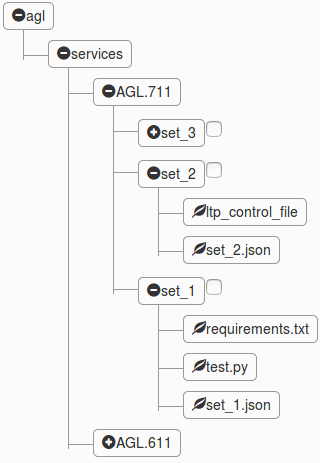
\includegraphics[width=0.82\linewidth]{images/test_suite.png}
	\caption{Test suite example}
    \end{minipage}
\end{figure}


\section{Architecture}
Ellida framework consists of two main parts - the actual application that provides all the functionality and metadata files. The metadata is organised as an OpenEmbedded layer and is used for integration with Poky. The framework is made up of several components that communicate through sockets and TCP connections. They can run on different machines and different networks as long as the settings are properly configured and the connections can be created. The main components are the \textbf{Engine}, the \textbf{Manager}, the \textbf{Controller} and the \textbf{Daemon}. They are loosely coupled to allow for as much flexibility as possible and enable scaling of the testing process.

In terms of communication and UI, relatively new but mature technologies were used such as ZeroMQ, WebSockets and Flask. The functional part of the framework is written only in Python, while the setup part uses Bitbake specific syntax that allows for a combination of Shell script and Python.

The \textbf{Engine} is at the centre of the communication system. Almost all communication has to pass through the Engine with no two components directly communicating with each other. The reason behind this design choice is that a centralized system is much easier to implement, monitor and control than a system where each component can communicate with every other component. It also enables a more predictable and manageable scaling process. Considering that Engines main task is to manage communication, the impact on overall efficiency is low enough not to outweigh the benefits. The \textbf{Manager} is responsible with the specification representation and keeps the test suite organized. The \textbf{Controller} is a user interface - the main I/O system and the \textbf{Daemon} is the part of the framework that runs on target distributions and executes the tests.

\subsection{Technologies}
\subsubsection*{ZeroMQ}
The backbone of the communication system is the ZeroMQ (ZMQ) library. It provides very efficient, highly scalable means of communication that abstracts most of the laborious setup usually required by network based systems. ZMQ is able to carry messages across inproc, IPC, TCP, TIPC, multicast and provides patterns recurrent in distributed systems such as push-pull and router-dealer. The testing framework uses a more common pattern - socket pair, and TCP connections. The Engine uses ZMQ polling to listen for multiple connections coming from different components.

\subsubsection*{Flask}
The Controller component is a web application with a Flask based backend. Flask is a Python web framework that is lightweight, very configurable and easy to setup. It is considered to be a microframework as it comes with only a couple of dependencies and only one development restriction - that the application project has a predefined structure. Its simplicity makes it an excellent choice for an application that needs to be as extensible as possible. The code base as well as the necessary setup are reduced, while the resource footprint is minimal. The setup is able to run without any delays on a very low powered, single core development board (RaspberryPi Zero).

Flask is based on two previously developed projects - Werkzeug toolkit and Jinja2 template engine. Werkzeug has a built-in web server and Jinja provides a flexible template system based on a mix of Python scripts and HTML code. It is a powerful and expressive combination suitable for frontends where content can be created procedurally, a good option for developers that need to focus more on the backend.

\subsubsection*{Bootstrap and WebSockets}
UIs frontend is based on the Bootstrap web framework and the WebSocket protocol. Bootstrap offers a set of predefined common graphical elements such as buttons and input forms that are easy to use and customise. WebSockets are a clean and efficient bridge between the frontend and the backend. Both Bootstrap and WebSocket can be integrated with a Flask application through community-made plugins (flask-bootstrap and flask-socketio).

\vspace{7mm}

The purpose of using this particular collection of technologies is to harness already existing open-source frameworks and tools as much as possible and focus the development effort on the main task - validating Linux distributions. Every choice is consistent with the ideal of a highly customisable, easy to use, well documented and high performing system.

\subsection{Components}

A testing framework that targets full distributions will naturally have to manage several very different operations. As a result, the proposed framework uses four distinct subsystems:
\begin{itemize}
\item The Engine - communication manager
\item The Daemon - test runner, available on the tested system
\item The Controller - UI, used by a tester to execute tests and receive results
\item The Manager - tool that keeps the internal representation of the specifications organised and up to date
\end{itemize}

\begin{figure}[h!]
  \centering
	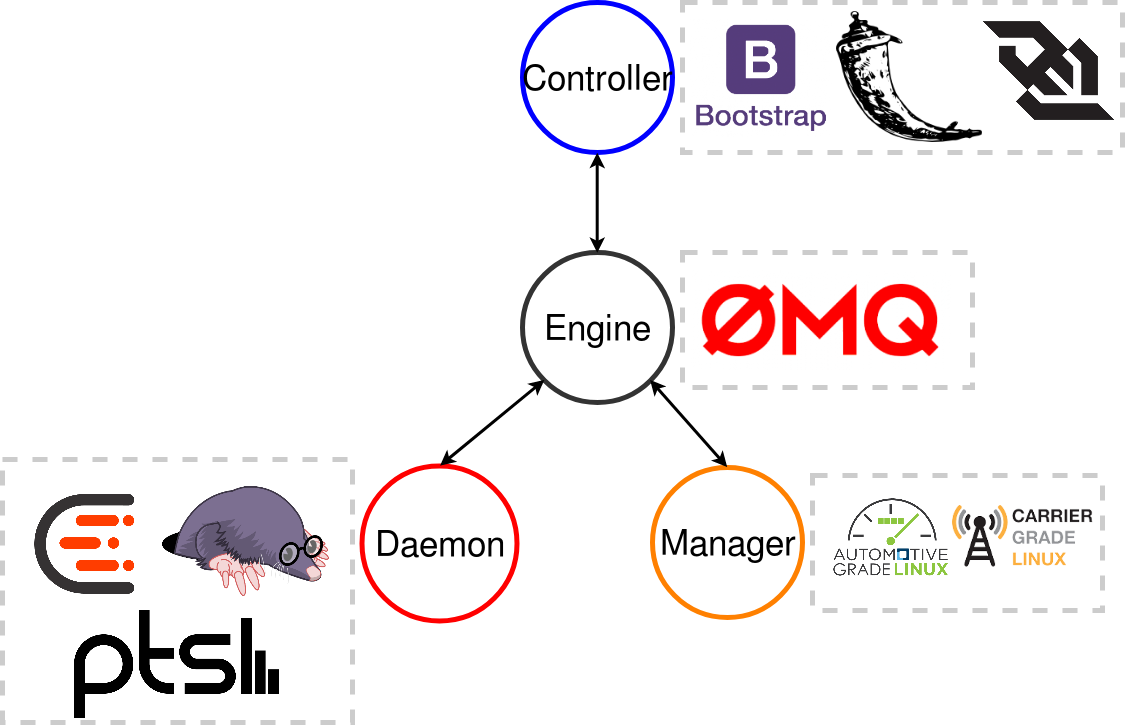
\includegraphics[width=\textwidth]{images/ellida_arch.png}
    \caption{Main components of Ellida framework}
\end{figure}

\subsubsection*{The Engine}
The engine is a central node of communication responsible for coordinating all the other components. It listens for messages and connections and relays them based on the the internal protocol. It is structured around a polling loop inside which specialised functions are called when particular messages arrive. Each function implements a certain part of the internal protocol and usually does as little processing work as possible. The functions only unpack the message, augment it with identification or protocol specific information and then send it to the destination. In the case of Daemon - UI communication the Engine is used to create a direct link between the two. The test results do not pass through the engine, this means that it is not burdened by the heaviest load in the system and the most important part of the communication benefits from less overhead.

The engine is meant to function as a publicly accessible service, ideally paired with an instance of UI, although this is not a requirement. It makes peer discovery easy (Controllers and Daemons) and can abstract away the Daemons, potentially turning the network of connected devices into a uniform resource for parallel testing on multiple targets.

\subsubsection*{The Controller}
Also referred to as the UI, it serves as the main input and output system. Considering that it is implemented as a Flask based web application it also fulfils one of the initial requirements of the project, that test control is available remotely. Although the system is referred as "user interface" it embodies one of the active nodes from the testing network. This means that the backend is just as important as the frontend.

In the current implementation of the communication protocol, one Controller can run tests on only one Daemon at a time. The user can select what part of the specification it intends to test and the information will be bundled together and sent to the target. When a user decides to run a set of tests on a Daemon (target device or VM), the Controller starts listening on a random port and notifies the Engine. The Daemon receives the identification details and creates a direct connection, the connection is only active while the tests run and ends after the Daemon had sent the results back.

\subsubsection*{The Daemon}
The Daemon is the part of the system that triggers the actual testing process. It uses provider modules to execute specific files and to gather the results. As the name suggests, it is intended to run as a daemon process and connects to an Engine instance. Selecting an Engine to connect to is done through a configuration file.

The Daemon is installed through the Yocto build system, in particular, through a Bitbake recipe. The program resides in the system as a globally accessible Python module. While running, the Daemon listens for messages from the Engine, reads the requests and uses a locally available test suite to search for the requested tests. 

\begin{figure}[h!]
  \centering
	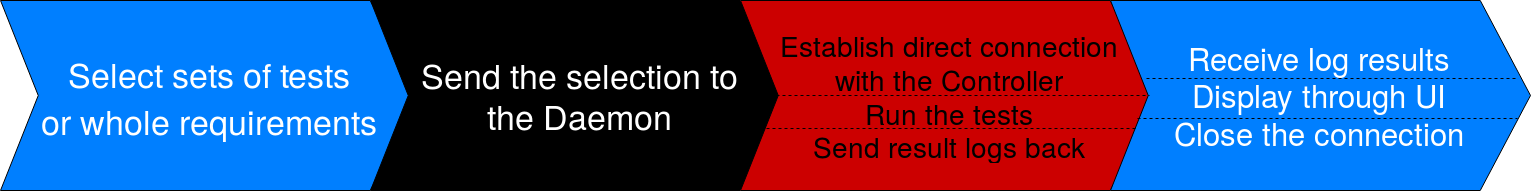
\includegraphics[width=\textwidth]{images/execution_flow2.png}
    \caption{Running a test suite}
\end{figure}

\subsubsection*{The Manager}
One of the more static parts of the framework, the Manager is a collection of parsers and methods for working with files. It can be used to get the latest version of a given specification, parse it and generate the abstract representation - a folder tree containing JSON files. The manager can also check the integrity of the test suite and report standard violations such as creating a test set with more than one provider.

\begin{figure}[h!]
  \centering
	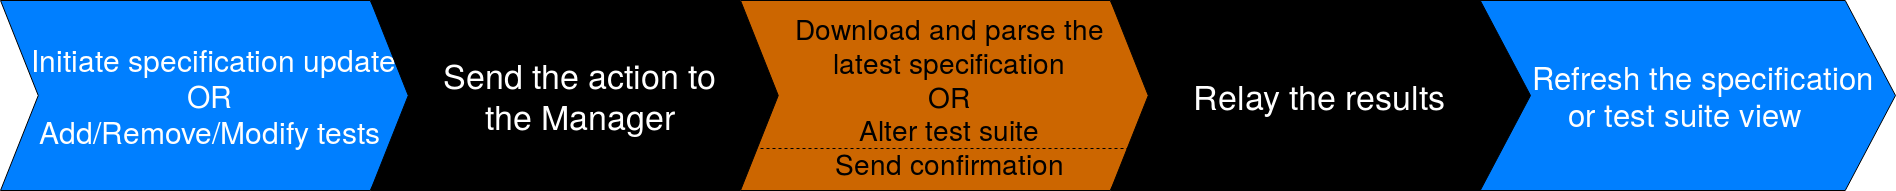
\includegraphics[width=\textwidth]{images/execution_flow1.png}
    \caption{Updating a specification or the test suite}
\end{figure}

\vspace{7mm}

Together, these four components fulfil the requirements of parsing and representing a specification, exposing test controls to the user, manage remote execution of tests, spawn test processes, and return test results.

\section{Yocto integration}

While the core functionality of the Ellida framework can be used on any type of system, for the more advanced features, mainly the providers, the target is expected to be a system generated with Poky. The providers are mostly Linux specific frameworks that require a minimal setup in order do be used. The Ellida framework requires only a Yocto specific setup as it comes embedded inside an OpenEmbedded layer (meta-ellida). The users have to install the layer and its dependencies (meta-oe and meta-python) in their current Yocto setup and run an installation script that appends dependencies to the target Yocto build folder. Bitbake will use the recipes inside the layer to install the Daemon Python project and will also include all the dependencies, mainly, the test providers.

The bitbake recipe contains a description for the standard Python package of the Daemon and setup commands for creating the test suite folder tree. The build system automatically executes the setup.py script and installs the package globally. The recipe for installing the Daemon can be found in the last section - Source code.


\chapter{Evaluation}

As stated in the introductory chapter, the framework proposal has one important purpose, to validate a Linux distribution based on a specification. It should provide the user with a measure of how compatible a given Linux based system is with one of the supported specifications. The evaluation chapter will try to determine to what extend the project meets these requirements, if it provides the expected functionality and finally, how it compares to the existing solutions.

The following list is a compilation of requirements either present in the projects description or based on the features already available in software with a similar purpose.

\begin{enumerate}
\item Enable a vendor of distributions to easily verify their compatibility with a specification
\item Develop an extensible system
\item Encapsulate the available Linux testing suites
\item Develop a scalable architecture
\end{enumerate}


\textbf{1. Enable a vendor of distributions to easily verify their compatibility with a specification}

The current state of the Ellida framework makes a specification available as a test suite and enables the tester to run tests for individual requirements. Therefore it offers a systematic and easy to track system with quantifiable results. In addition, the process is made simple from two points of view.

Firstly, it offers a high degree of automation for the setup stage through integration with Yocto. If a large enough set of providers are supported by Ellida, the setup can become cumbersome, especially if it has to be repeated on many different variants of a system. A Yocto based setup will also guarantee that the Daemon component and the test suite have a uniform setup across all systems, eliminating trivial problems such as path errors or missing dependencies. Since the framework is defined as a separate OpenEmbedded layer and as a set of dependencies, Yocto can automatically manage the aforementioned laborious task.

Secondly, by abstracting away the details of a specification and formatting the test suite so that it mirrors the specifications, it becomes easy to track compatibility rate as well as overall coverage. An attribute difficult to asses in practice can eventually become a numeric value.

\textbf{2. Develop an extensible system}

The "extensibility" trait is attributed both to the test suite and the technical system. The test suite is extensible in a sense that it has a permissive format, yet the structure is dictated by the specification. Furthermore, by defining every requirement as a list of test sets, each set with a specific provider, the tester is free to use as many tests and tools as possible to test a single requirement. The metadata uses the ubiquitous JSON format, both easy to parse and human readable.

The extensibility of the technical system is more limited from an architectural point of view. The main components are fixed, as well as their behaviours, but the system is very modular and the requirements are simple enough not to require any change - connect to a target and run a set of tests. From a functional point of view, the Daemon, the Manager and the Controller are very easily extensible.

\begin{itemize}
\item \textbf{The Daemon} encapsulates a provider module, which is made of class abstractions for open source testing tools. To add a new provider, a new abstraction class needs to be written and added to the module. The effort is small considering the extensive functionality gained, but some tools are more difficult to use than others. One aspect that influences the effort of adding providers is their availability within the OpenEmbedded collection of software.
\item \textbf{The Manager} contains a set of parsers that can output the representation of a specification. The starting point for supporting a new specification is to write a parser class and integrate it. However, the obvious bulk of the work will come afterwards when populating the new test suite.
\item \textbf{The Controller} or the UI, uses software that benefits from a large community, Flask is notoriously easy to extend or modify and a large collection of plugins is already available. This makes it easy to add advanced functionality such as databases or visualization tools.
\end{itemize}

\textbf{3. Encapsulate the available Linux testing suites}

As discussed in previous chapters, testing tools and frameworks from the open source community are abstracted as \textbf{providers}. Currently the implementation only supports three such systems - LTP, Image Tests and Core - basic functionality that enables the execution of Python scripts. However, the model allows integration for any tool.

\textbf{4. Develop a scalable architecture}

By distributing functionality among different components communicating through TCP connections the framework can fit within a wide range of testing setups and can take various forms so that it makes better use of resources. It can run on a single computer or spread functionality across multiple nodes. Since using more Daemons at once is not yet implemented, the topic of distributed testing is further developed in the \textbf{Further Developments} chapter.

\section{Performance}
The current implementation allows a user to run a small dummy set of tests on any Linux target on which a Daemon instance runs. The communication protocol currently supports running tests on one Daemon at a time. Given this limitation it is difficult to asses the framework performance-wise. The communication overhead is negligible for such a low packet traffic and the data passing through the system is minimal - JSON formated test sets and text log files. The interface runs smoothly with very rare performance drops and no obvious glitches on any of the major browsers.

In terms of resource footprint the Flask backend uses less than 8MB or memory. During a light stress test with close to 100 TCP connections active, a bandwidth usage of less than 4Mbit/s and an average of four requests per second, the CPU usage remained under 50\%. The test was run on a very low spec board - a Rapsberry Pi Zero W with one ARMv7 1GHz core and 512MB of memory. The reduced maximum bandwidth is in part attributed to the slow WiFi connection.

No extensive stress tests were run for one particular reason, it would not test the architectural limits of the system, but the technical limits of the technologies used such as the Flask backend, the Javascript/Python implementation of WebSockets, ZeroMQ network etc.

The most relevant metrics are how suitable the framework is for the task and how much faster the development of embedded systems becomes by using it. Unfortunately, developing a full test suite that covers most of a specification is a very laborious and subjective task. Furthermore, even if the system was complete - provided distributed testing and a complete test suite - the technical performance of the framework itself would not be the bottleneck in terms of time. The overhead added by the system is negligible in comparison to the network communication times and more importantly, the tests run times. The functionality was tested with a small set of LTP control files that ran up to three common tests such as memory allocation and filesystem operations on several types of systems - VMWare and Qemu VMs and x86 Ubuntu Linux.

\section{Limitations}

While the model is intended to be powerful through simplicity, the current technical implementation does not use it at full potential. Several limitations spawn from the shallow implementation of the communication protocol, namely - the system is not fault tolerant, the UI can only use one Daemon at a time and blocks while tests are being run. The scalability is hindered also by the lack of a formal system that allows tests to be run in parallel on the same system. The current implementation does not contain any information about how tests relate to one another. Therefore, running multiple tests on the same system can not be achieved safely due to the influence some tests might have on others. Benchmarking tests for instance could alter the results of any other type of test.

Perhaps the most crippling missing part are the test suites themselves. Though arguably not part of the framework, a test suite that validates an entire specification is difficult to write. The next chapter develops on a profile based concept that could ease the task by making it a community effort and share the progress and work between individual developers or vendors.

The framework is highly dependable on the Yocto software stack. Therefore, a notable limitation is the OpenEmbedded software collection that is the source of providers. If a tool is intended to be used and is not already in the OE collection, then it first has to be integrated through an OE layer. However, the benefits of using Yocto and OE and the extended documentation about OE layers lead to a limited impact on development time.

\chapter{Further developments}

\section{Distributed testing}

In order to scale, the framework should be able distribute tests to a network of Daemon nodes (target distributions). One way of doing so is by using "local networks". It is defined as a collection on Daemons and the Engine instance connected to them. The Engine should make the set of Daemons available to any Controller that joins its network. Through the UI a tester can then select not only the tests to be run, but also the targets. The initial implementation could simply broadcast the set of tests to all selected Daemons, but with a good enough UI, test selection could also be Daemon specific. The results could be provided as a bundle by the Engine, or sent directly to the Controller which will wait for them.

\begin{figure}[h!]
  \centering
	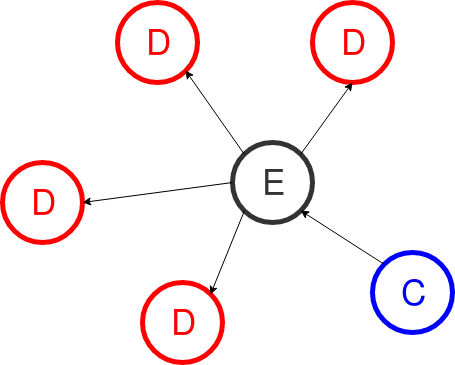
\includegraphics[width=0.4\textwidth]{images/local.png}
    \caption{Example of a local network}
\end{figure}

In order to make the system scalable not only with the number of target devices, but also with the number of parallel instances of Daemons running on the same distribution, a dependency tracking and checking system between tests must be implemented. 

\subsection{Access control and network labels}

By using local networks defined as a set of Daemons and an Engine, an access control system could de implemented that uses Controller identification and defines what access rights should be offered.

Additional functionality can be provided by labeling. A local network could be limited to a specific task - run tests for a single requirement on multiple types of targets or run tests from the same provider even if they test different requirements. 

\section{Test profiles}

When writing a test suite, a vendor or community will have subjective views about what validation means, or when a requirement is truly validated. This can lead to different test suites for the same specification. These different branches could be viewed as "profiles" of the same specification and would benefit all if brought under a publicly available service. Vendors could start by building on already existing suites while the rest of community will be able to judge how well the specification is tested. The process will be accelerated and will become very transparent. From a technical point of view, it would mean that the test suites available on the targets and used by the Daemons will need a versioning system and identification.

% \begin{figure}[h!]
%   \centering
% 	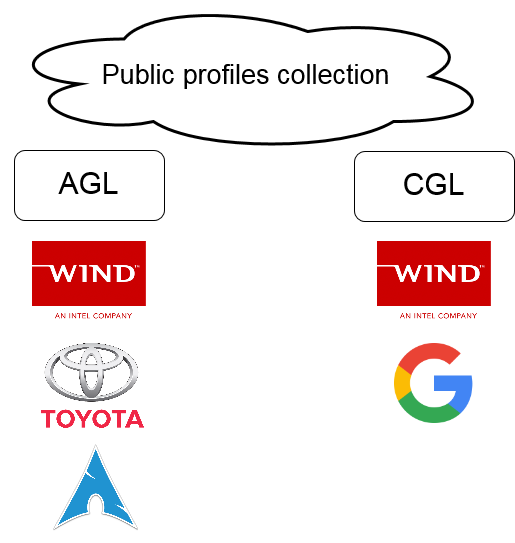
\includegraphics[width=0.5\textwidth]{images/profiles.png}
%     \caption{A public profile repository}
% \end{figure}

\chapter{Conclusions}

To sum up all the aspects presented in the previous chapters, the framework proposal is more of an architectural proposal accompanied by a functional but limited software representation. The solution focuses on the fundamental requirement - being able to validate a Linux distribution based on a specification - and offers the functionality through a flexible model and simple design. The abstraction of specifications, quantification of compliance and the extensive use of open-source tools to create a convenient and useful framework is the main achievement of the project.

The technical implementation uses lightweight, efficient and extensible open source projects. 

Ellida is not supposed to be a more efficient solution, but to provide high level features

 
% Include appendix
\appendix
\chapter*{Source code}
\begin{lstlisting}[caption = {Daemons Bitbake recipe}]
DESCRIPTION = "Daemon process that manages communication between the engine and the target"
SECTION = "ellida"
LICENSE = "MIT"
SRC_URI = "file://setup.py \
            file://ellida_daemon.py \
                file://ellidadaemon/__init__.py \
                file://ellidadaemon/settings.py \
                    file://ellidadaemon/providers/__init__.py \
                    file://ellidadaemon/providers/ltp_provider.py \
                    file://ellidadaemon/providers/provider.py \
                file://ellidadaemon/daemon.py"
SRC_URI += "file://ellida_tests"
PYTHON_2_LIBS = "/usr/bin/python2.7/site-packages/"
PYTHON_3_LIBS = "/usr/bin/python3.5/site-packages/"
S = "${WORKDIR}"
TEST_LOG = "/opt/logs"
TEST_DST = "/opt/"
inherit setuptools

RDEPENDS_${PN} += "\
        python-pyzmq \
        python-daemonize"
do_install_append() {
    rm -rf ${D}${TEST_DST}
    install -d ${D}${TEST_DST}
    install -d ${D}${TEST_LOG}
    cp -r ${S}/ellida_tests ${D}${TEST_DST}
    install -d ${D}${bindir}
    install -m 0755 ellida_daemon.py ${D}${bindir}
}
FILES_${PN} += "/opt/ellida_tests/*"
FILES_${PN} += "/opt/logs"
\end{lstlisting}


% Include list of figures
\clearpage
\addcontentsline{toc}{chapter}{List of figures}
\listoffigures

% Include bibliography
% Manually add Bibliography to the TOC
\clearpage
\addcontentsline{toc}{chapter}{Bibliography}

% Bibliography starts here
\begin{thebibliography}{99}
	\bibitem{bk:primer}
		{Daiane Angolini, Otavio Salvador  --
			\emph{Yocto for Embedded Linux Development Primer} -- 2014 -- Packt}
    \bibitem{bk:cookbook}
		{Alex Gonzalez  --
			\emph{Embedded Linux Projects Using Yocto Project Cookbook} -- 2015 -- Packt}
    \bibitem{bk:guide}
		{Alexandru Vaduva  --
			\emph{Learning Embedded Linux Using the Yocto Project} -- 2015 -- Packt}
\end{thebibliography}


\end{document}